\section{Sistemi retroazionati: proprietà e analisi asintotica}

\subsection{Schemi a blocchi}
I sistemi complessi possono essere rappresentati mediante l'uso di schemi
a blocchi, alcuni esempi dei blocchi pi\`u comuni:

\begin{figure}[h!]
    \centering
    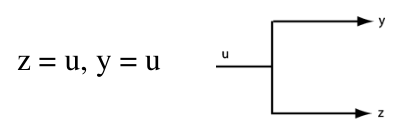
\includegraphics[width=0.3\linewidth]{images/blocchi_diramazione.png}
    \caption{Blocchi di diramazione}
    \label{fig:diramazione}
\end{figure}

\begin{figure}[h!]
    \centering
    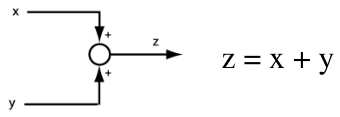
\includegraphics[width=0.3\linewidth]{images/blocchi_sommanti.png}
    \caption{Blocchi sommanti}
    \label{fig:sommanti}
\end{figure}


\subsection{Regole di riduzione}
\begin{figure}[h!]
    \centering
    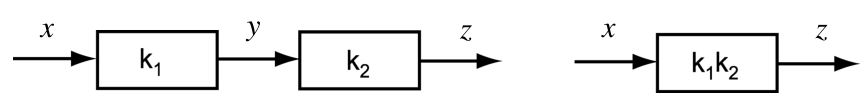
\includegraphics[width=0.3\linewidth]{images/riduzione_cascata.png}
    \caption{Riduzione di blocchi in cascata}
    \label{fig:cascata}
\end{figure}

\begin{figure}[h!]
    \centering
    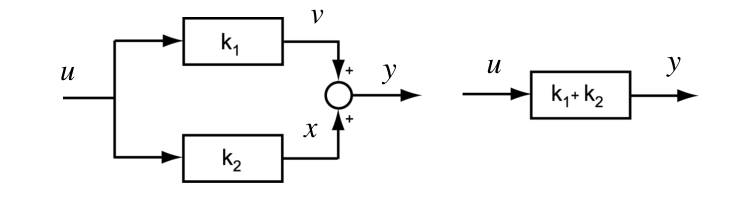
\includegraphics[width=0.3\linewidth]{images/riduzione_parallelo.png}
    \caption{Riduzione di blocchi in parallelo}
    \label{fig:parallelo}
\end{figure}


\begin{figure}[h!]
    \centering
    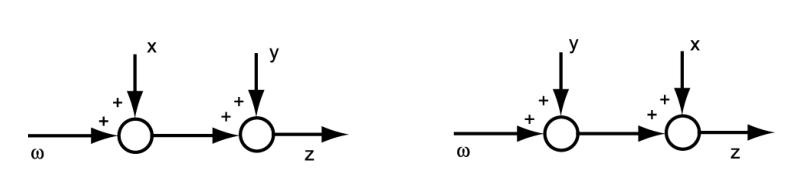
\includegraphics[width=0.3\linewidth]{images/scambio_giunzioni_sommanti.png}
    \caption{Scambio di giunzioni sommanti}
    \label{fig:scambio_sommanti}
\end{figure}


\begin{figure}[h!]
    \centering
    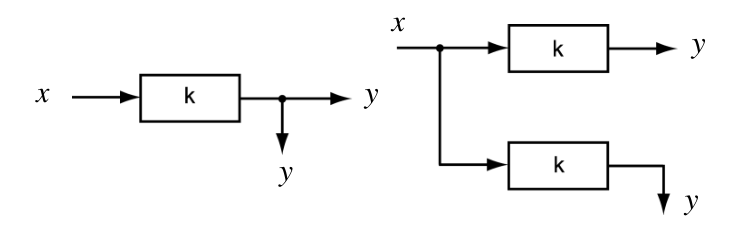
\includegraphics[width=0.3\linewidth]{images/spostamento_prelievo_segnale.png}
    \caption{Spostamento di prelievo di segnale a monte di un blocco}
    \label{fig:spostamento_prelievo_monte}
\end{figure}


\begin{figure}[h!]
    \centering
    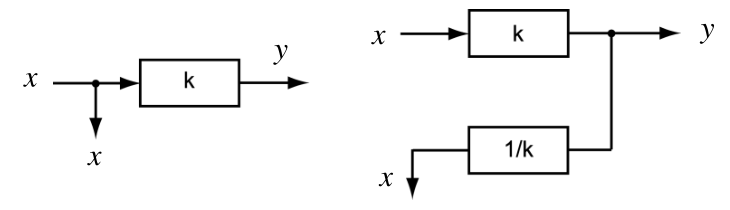
\includegraphics[width=0.3\linewidth]{images/spostamento_prelievo_segnale_a_valle.png}
    \caption{Spostamento di prelievo di un segnale a valle di un blocco}
    \label{fig:spostamento_prelievo_valle}
\end{figure}

\begin{figure}[h!]
  \centering
  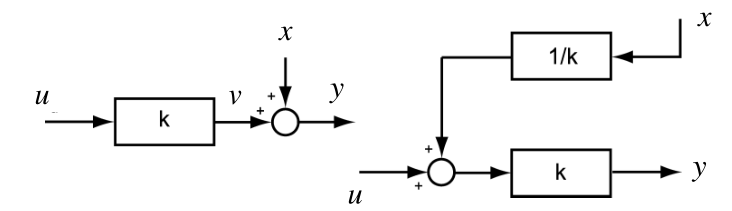
\includegraphics[width=0.3\linewidth]{images/spostamento_giunzione_a_monte.png}
  \caption{Spostamento di giunzione sommante a monte di un blocco}
  \label{fig:spostamento_giunzione_monte}
\end{figure}



\begin{figure}[h!]
  \centering
  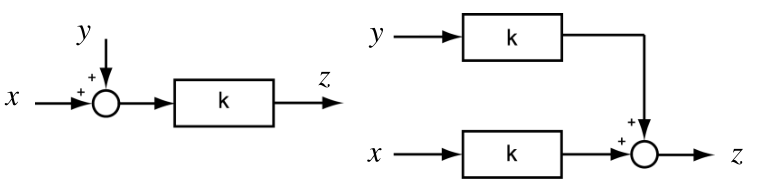
\includegraphics[width=0.3\linewidth]{images/spostamento_giunzione_a_valle.png}
  \caption{Spostamento di giunzione sommante a valle di un blocco}
  \label{fig:spostamento_giunzione_valle}
\end{figure}


\begin{figure}[h!]
  \centering
  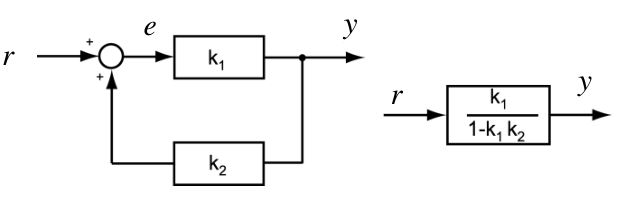
\includegraphics[width=0.3\linewidth]{images/eliminazione_anello.png}
  \caption{Eliminazione di un anello}
  \label{fig:eliminazione_anello}
\end{figure}



\newpage
\subsection{Proprietà generali dei sistemi in retroazione}
\begin{figure}[h!]
  \centering
  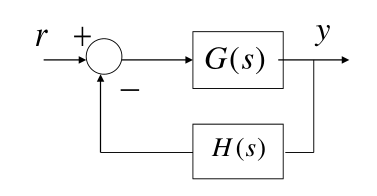
\includegraphics[width=0.3\linewidth]{images/retroazione.png}
  \caption{Schema a blocchi di un sistema in retroazione}
  \label{fig:retroazione}
\end{figure}


La funzione di trasferimento risulta:
\begin{align}
  \text{FDT} &= \frac{\text{fdt del percorso diretto}}{1 + \text{guadagno ad anello}} \\
  &= \frac{G(s)}{1 + G(s)H(s)}
\end{align}

Osservazioni:
\begin{itemize}
  \item Un guadagno di anello elevato rende (relativamente) 
        insensibile la f.d.t. del sistema retroazionato a variazioni della 
        f.d.t. del sistema controllato
  \item Variazioni della f.d.t. nella catena di retroazione si 
        riverberano senza attenuazione in variazioni della f.d.t. del sistema 
        retroazionato
\end{itemize}


\subsection{Attenuazione dei disturbi}
Se il guadagno di anello è elevato il rapporto segnale/disturbo si eleva
all’incirca del medesimo fattore passando dallo schema in catena aperta a
quello in catena chiusa. Quindi, a parità di segnale utile, il disturbo viene
grandemente attenuato nel sistema in retroazione


\subsection{Allargamento della banda passante}

Un guadagno di anello elevato comporta un allargamento della banda passante.

\subsection{Analisi a regime dei sistemi in retroazione}

\begin{figure}[h!]
  \centering
  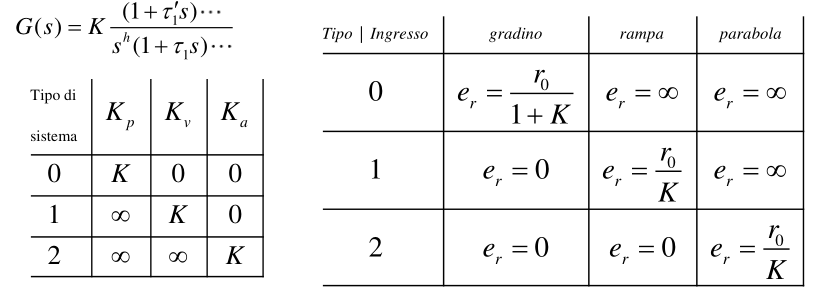
\includegraphics[width=0.5\linewidth]{./images/analisi_regime_retroazione.png}
  \caption{Analisi a regime dei sistemi in retroazione}
  \label{fig:analisi_regime_retroazione}
\end{figure}



